%!TEX program = lualatex
% LTeX: language=de-DE
\documentclass[a5paper]{scrartcl}
\usepackage[utf8]{luainputenc}
\usepackage{emoji}
\usepackage[
	typ=ab,
	fach=Informatik,
	lerngruppe=6,
	zitate=quotes,
	namensfeldAnzeigen,
	datumAnzeigen,
  seitenzahlen=keine,
	lizenz=cc-by-sa-4,
	farbig,
	module={Symbole,Lizenzen}
]{schule}
\renewcommand{\familydefault}{\sfdefault}
\usepackage[left=2cm,right=2cm,top=1cm,bottom=1cm,includehead,includefoot]{geometry}

\ifoot{v2023-12-17}
\cfoot{}
\ofoot{\lizenzSymbol}

\usepackage{pgfpages}                                 % <— load the package
  \pgfpagesuselayout{2 on 1}[a4paper,landscape, border shrink=5mm] % <— set options
%
%\usepackage{atbegshi}
%  % duplicate the content at shipout time
%  \AtBeginShipout{
%    \pgfpagesshipoutlogicalpage{1}\copy\AtBeginShipoutBox
%    \pgfpagesshipoutlogicalpage{2}\box\AtBeginShipoutBox
%    \pgfshipoutphysicalpage
%  }

\usepackage{wrapfig}

\title{Codierung von Daten: B6-Code}
\author{Mike Barkmin}
\date{Datum: \hspace{1.5cm}}

\begin{document}
\subsection*{Wie kann mit dem B6-Code ein Wort codiert und decodiert werden?}

%\begin{wrapfigure}[7]{r}{0.4\textwidth}
%  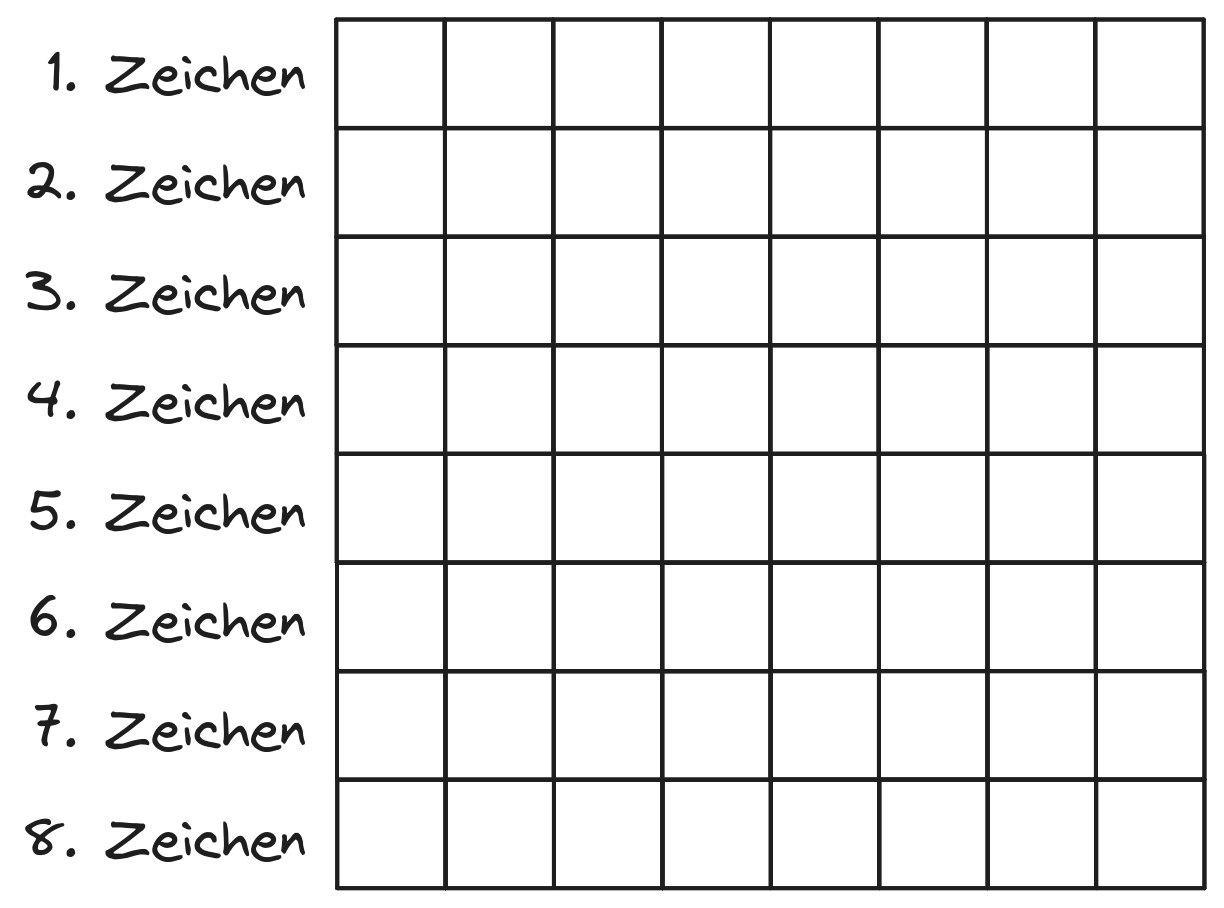
\includegraphics[width=0.4\textwidth]{./b6code-struktur.excalidraw.png}
%\end{wrapfigure}

Für den B6-Code muss jedes Zeichen des Wortes als Binärzahl codiert werden. Dazu wird die ASCII-Tabelle verwendet. Danach wird die Binärzahl in Pixel umgewandelt. Jede Zeile des B6-Codes enthält die Pixelcodierung des Zeichens.

\begin{center}
	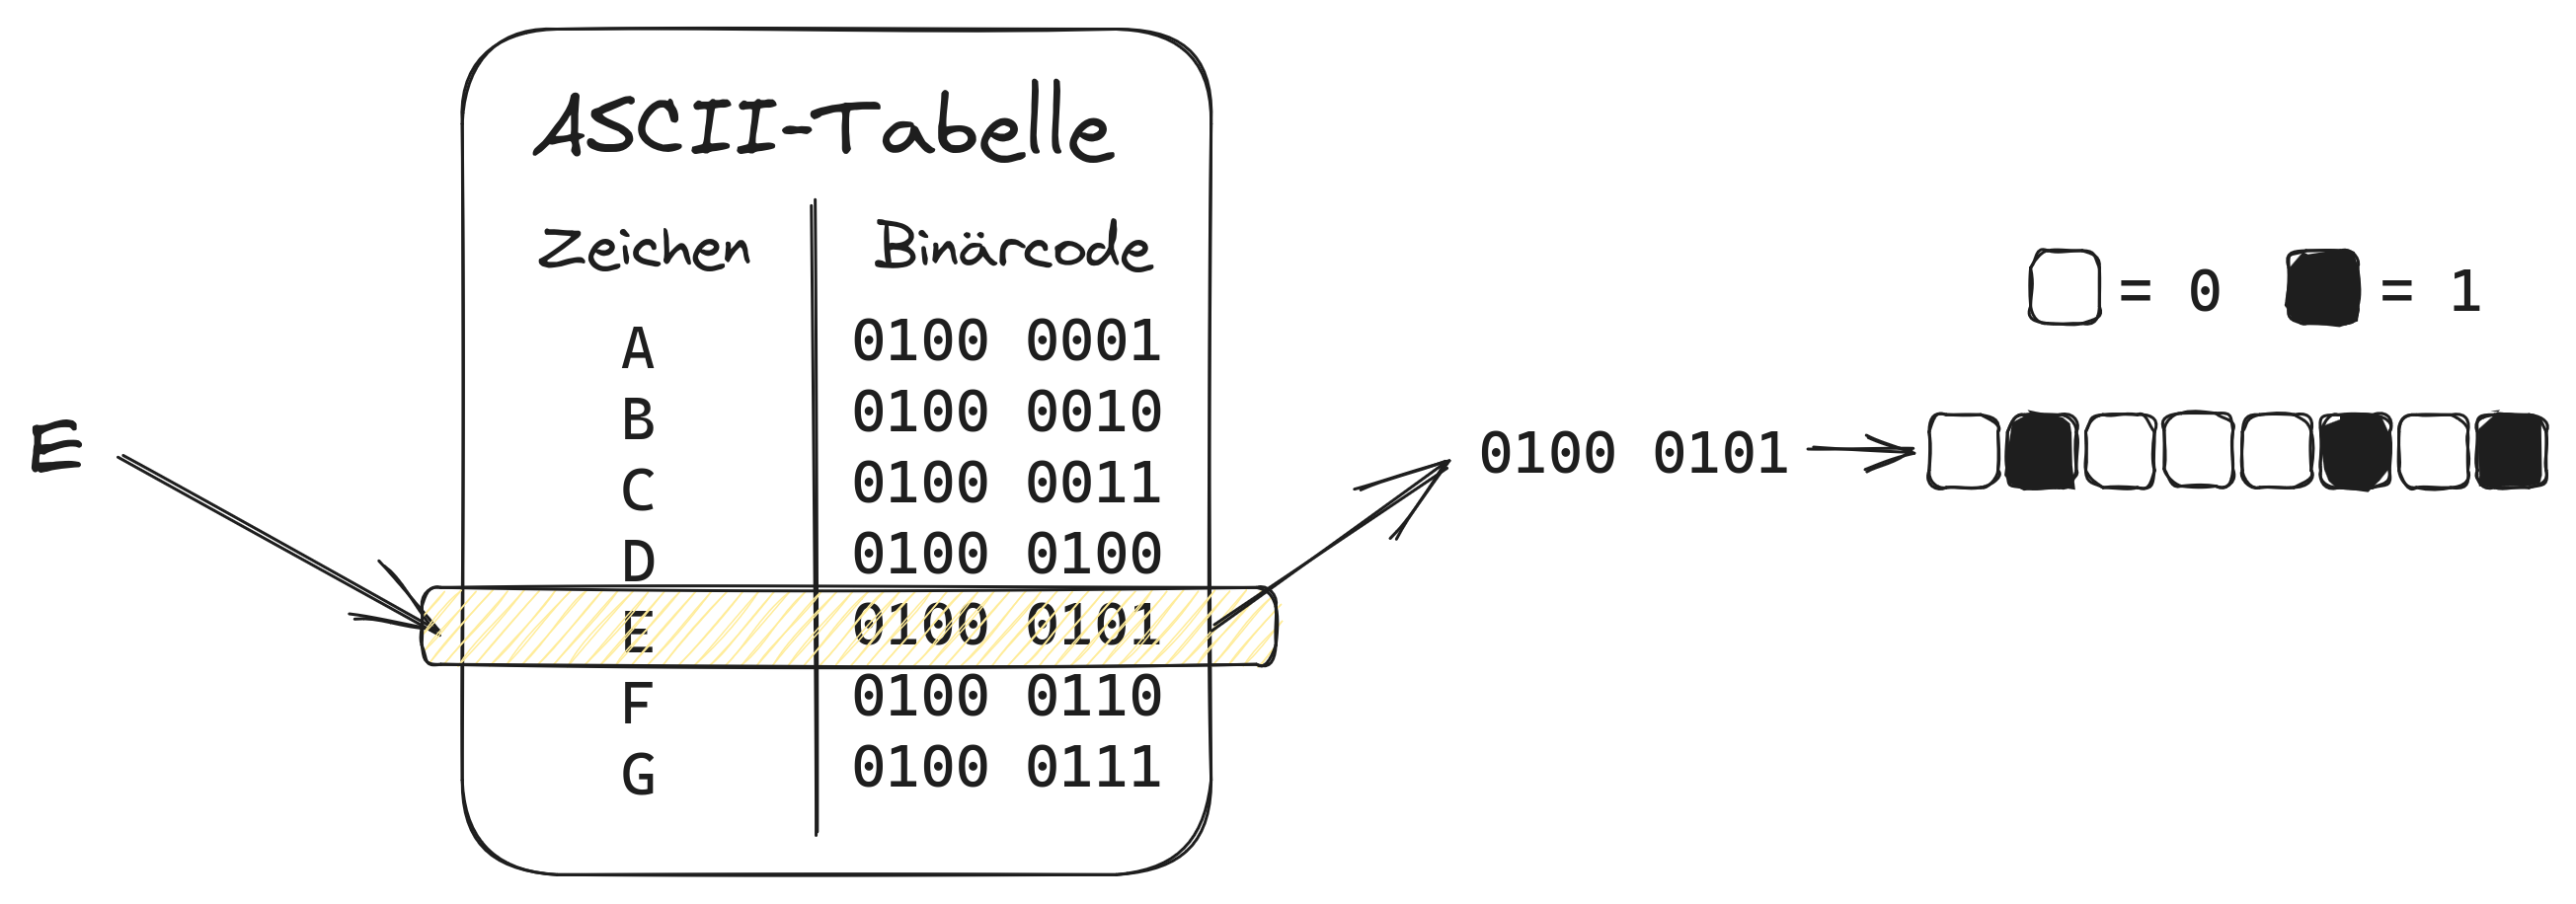
\includegraphics[width=0.9\linewidth]{./zeichen-zu-pixel.excalidraw.png}
\end{center}


\begin{aufgabe}
	\begin{teilaufgaben}
		\teilaufgabe \emoji{bust-in-silhouette} Codiere das Wort auf deinem Zettel mit dem B6-Code.
		\teilaufgabe \emoji{bust-in-silhouette} Tausche deine Codierung mit deinem/deiner Partner:in und decodiere den B6-Code.
		\teilaufgabe \emoji{busts-in-silhouette} Überprüft eure Ergebnisse gegenseitig.
	\end{teilaufgaben}
\end{aufgabe}

\newpage

\subsection*{Wie kann beim Dekodieren der Anfang des B6-Codes erkannt werden?}

\begin{center}
	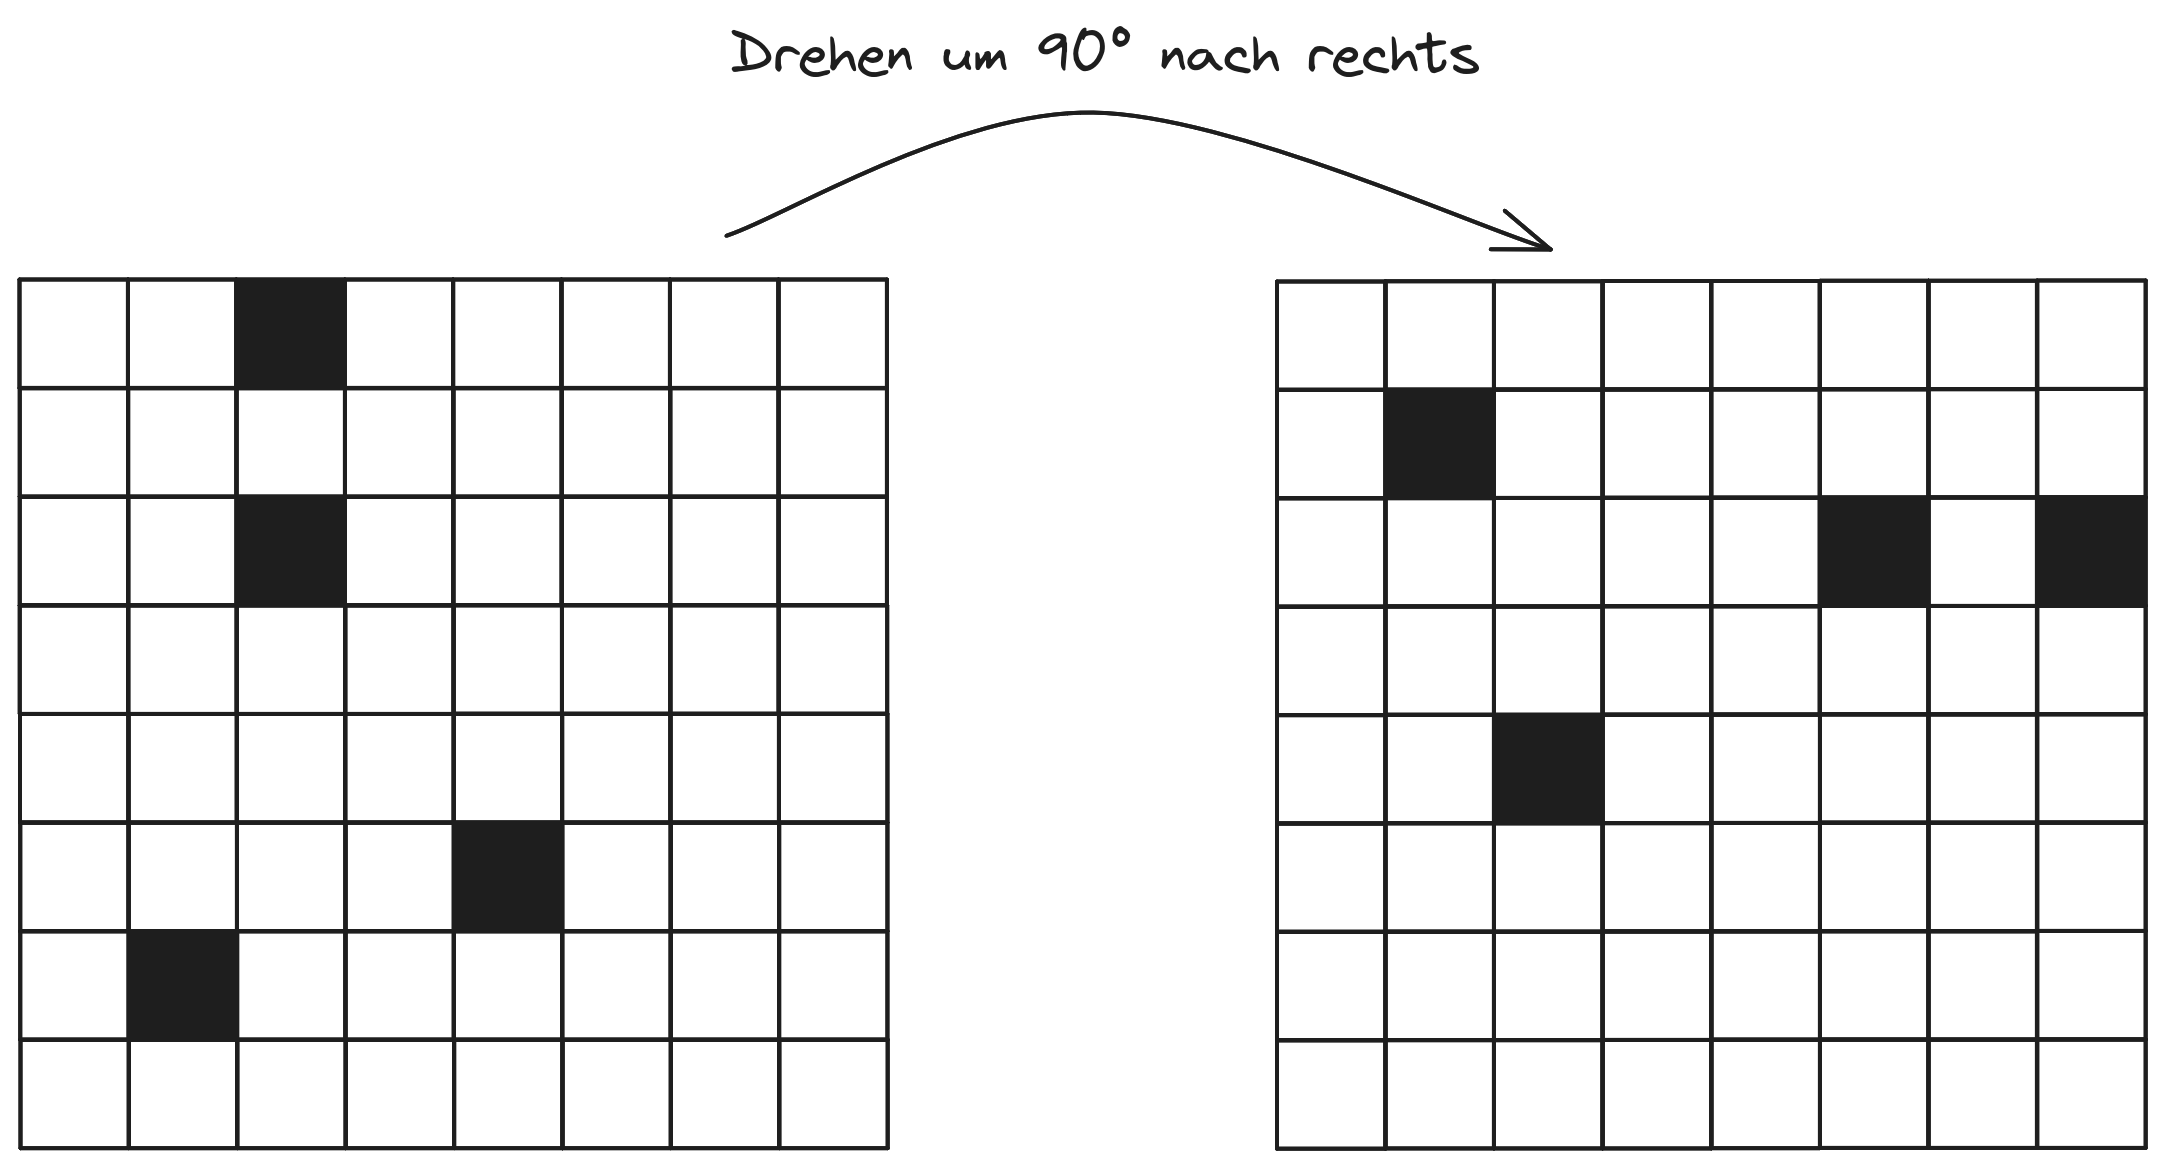
\includegraphics[width=0.9\linewidth]{./b6code-drehen.excalidraw.png}

\end{center}
\begin{aufgabe}
	\begin{teilaufgaben}
    \teilaufgabe \emoji{busts-in-silhouette} Dreht eure B6-Codes nach rechts und decodiert diesen erneut. Wenn ein Binärcode nicht in der ASCII-Tabelle zu finden ist, dann decodiert ein Leerzeichen (leere Stelle). Notiert was ihr dabei feststellt.
		\teilaufgabe \emoji{busts-in-silhouette} Entwickelt eine Möglichkeit, wie der Anfang des B6-Codes erkannt werden kann. Notiert dazu ein bis zwei Sätze.
	\end{teilaufgaben}
\end{aufgabe}

\newpage

\subsection*{Wie kann der B6-Code robuster gemacht werden?}

\begin{center}
	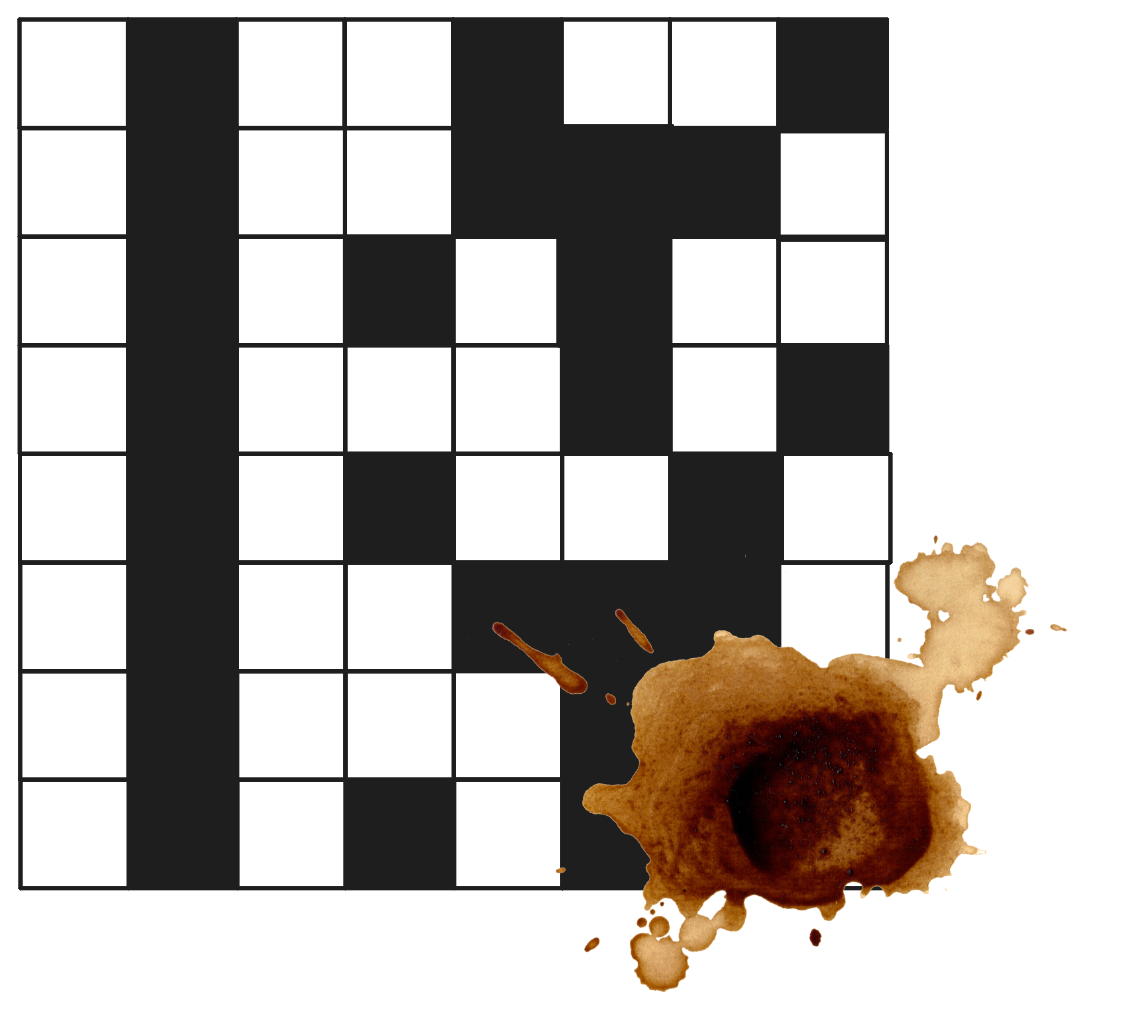
\includegraphics[width=0.9\linewidth]{./b6code-fehler.excalidraw.png}
  \footnotesize{B6-Code des Wortes \enquote{INTERNET} mit einem Kaffeefleck}
\end{center}

\begin{aufgabe}
	\begin{teilaufgaben}
		\teilaufgabe \emoji{busts-in-silhouette} Beschreibt welche Folgen es für das Decodieren hat, wenn ein Pixel unlesbar sind.
		\teilaufgabe \emoji{busts-in-silhouette} Findet Ideen, wie der B6-Code weniger anfällig gegenüber solchen Fehlern gemacht werden kann.
	\end{teilaufgaben}
\end{aufgabe}

\newpage

\subsection*{Wie kann der B6-Code lesbarer für einen Computer gemacht werden?}

Wenn eine große weiße Fläche enthalten oder der Code zu regelmäßig ist, dann ist es für einen Computer schwerer diesen zu lesen. Deshalb werden sogenannte Masken verwendet.

Eine Maske wird über den B6-Code gelegt. Ein weißes Feld in der Maske bedeutet, dass das betreffende Feld seine Farbe behält, bei einem schwarzen Feld wird die Farbe umgekehrt.

\begin{center}
	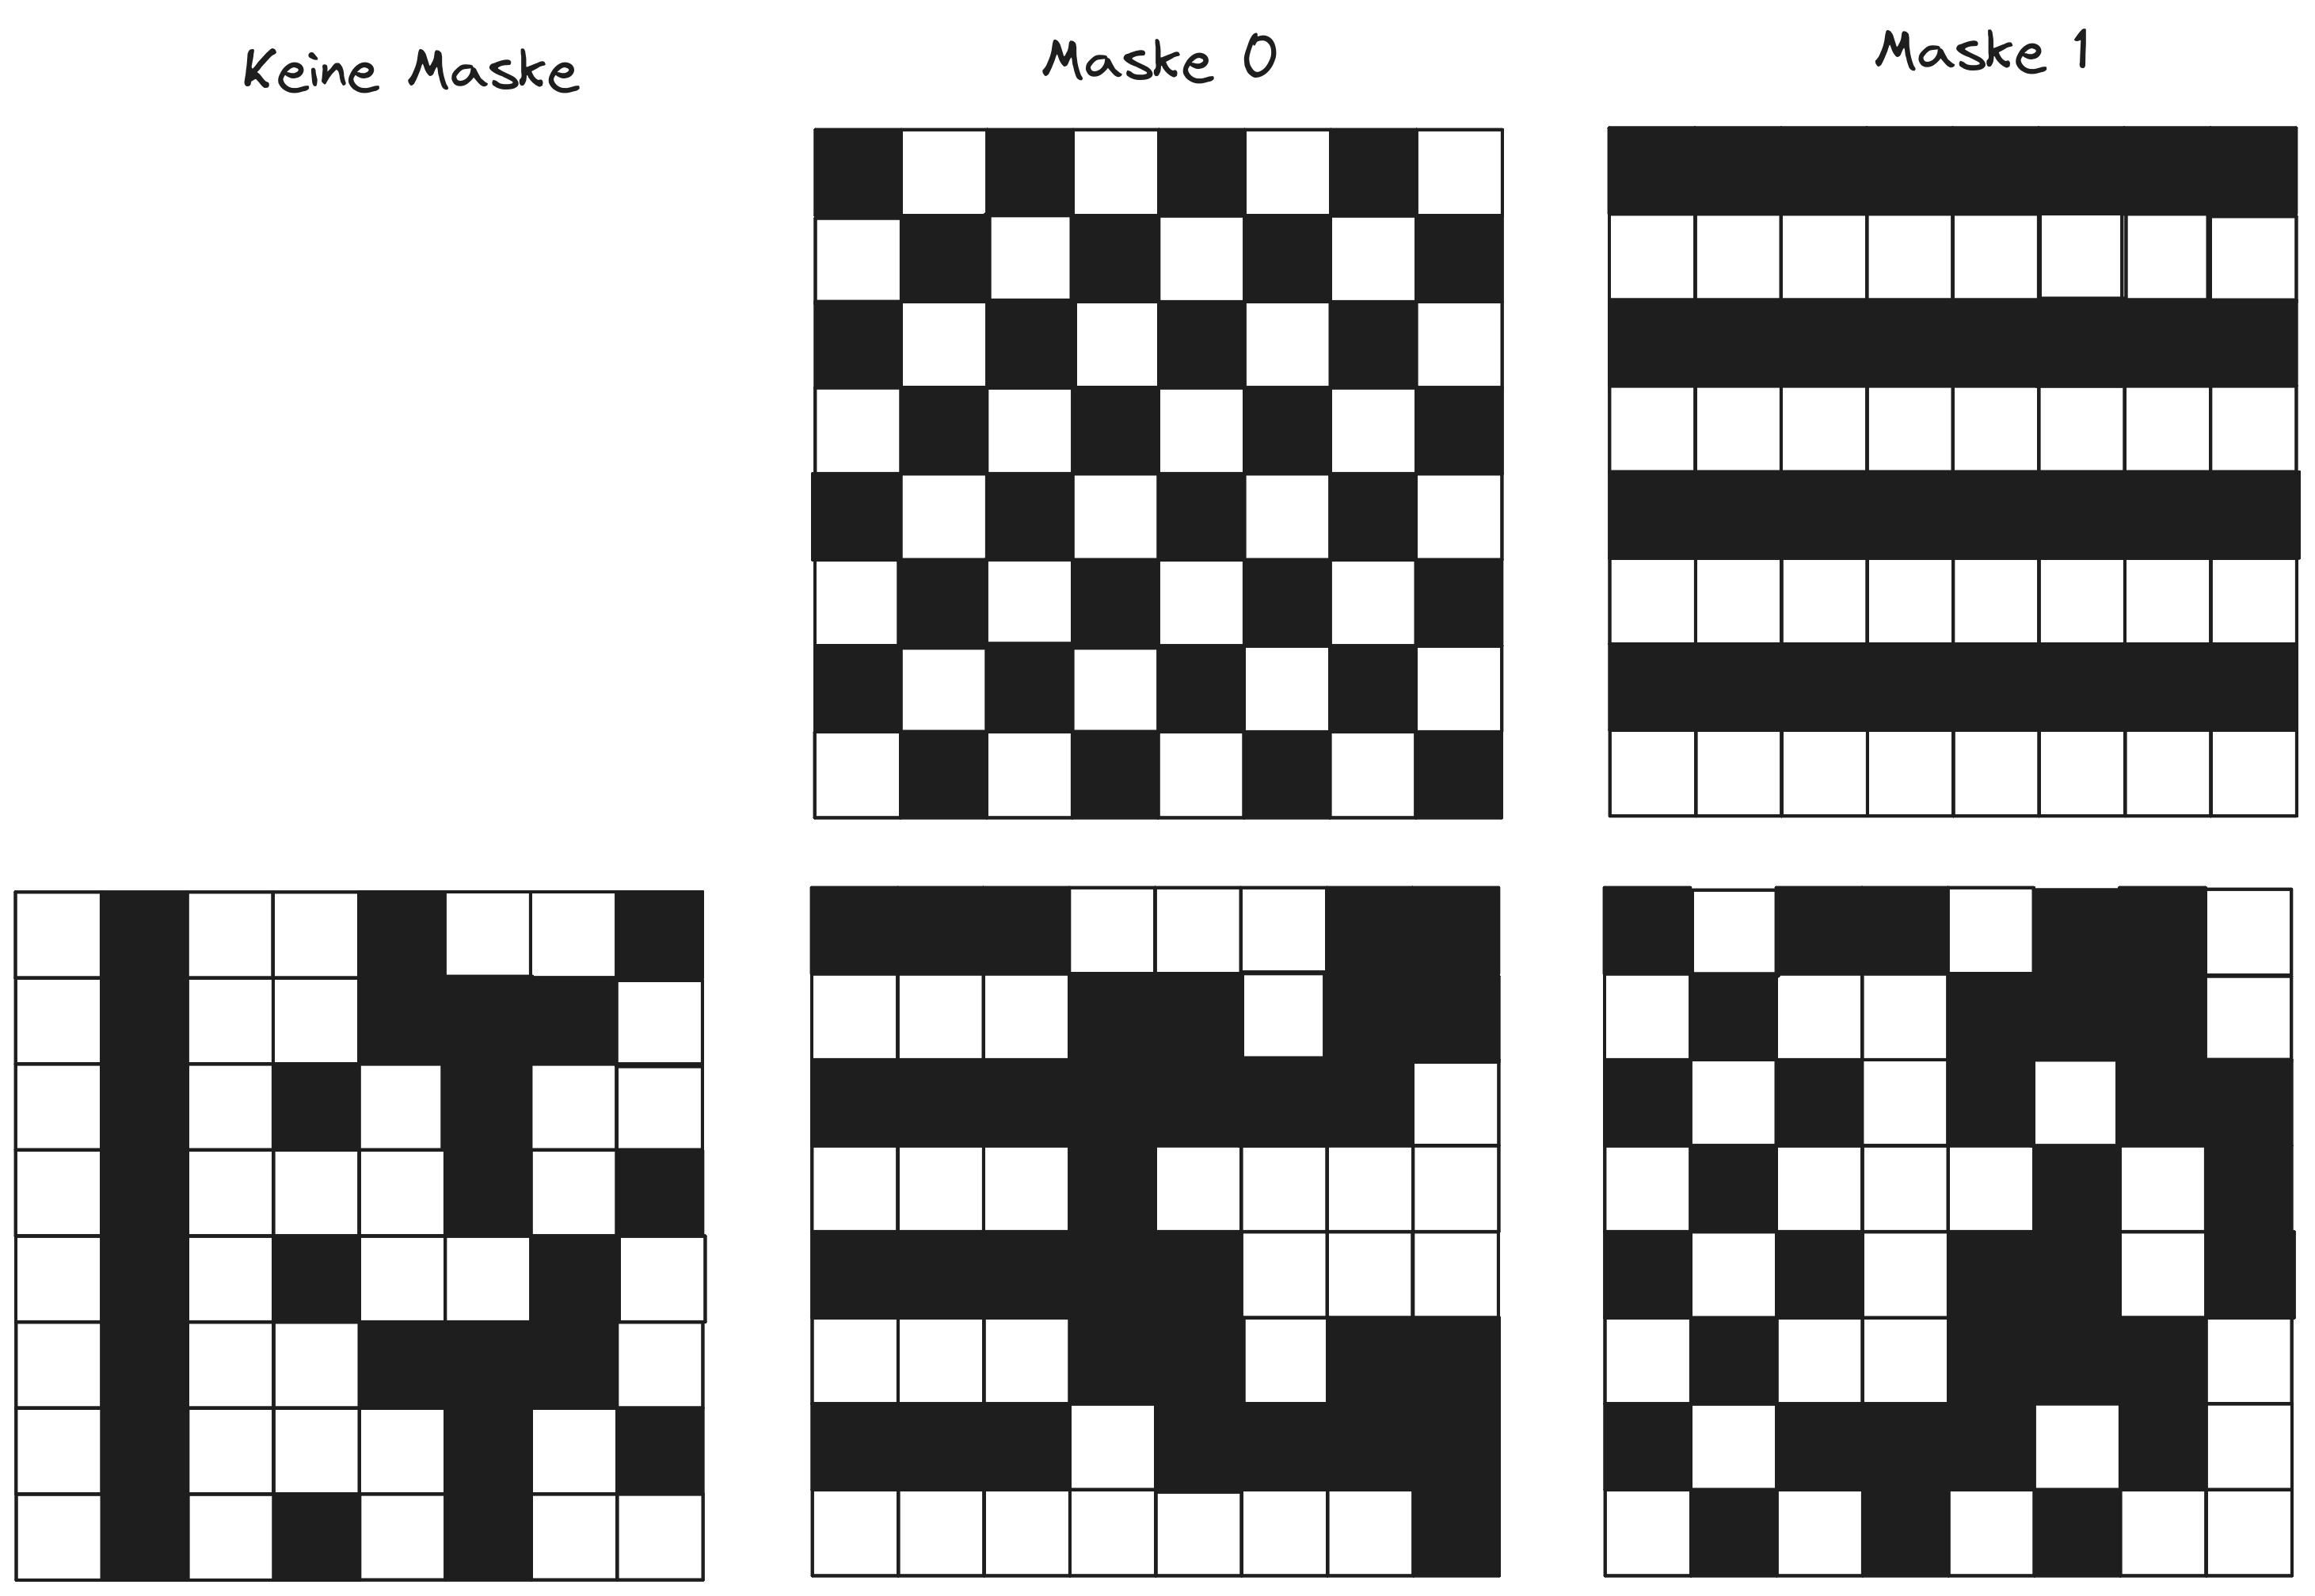
\includegraphics[width=0.8\linewidth]{./b6code-maske.excalidraw.png}
\end{center}

\begin{aufgabe}
	\begin{teilaufgaben}
		\teilaufgabe \emoji{busts-in-silhouette} Beurteilt, welche Maske sich hier am besten eignet.
		\teilaufgabe \emoji{busts-in-silhouette} Findet Ideen, wie im B6-Code gespeichert werden kann welche Maske benutzt wurde.
	\end{teilaufgaben}
\end{aufgabe}

\end{document}
